%%%%%%%%%%%%%%%%%%%%%%%%%%%%%%%%%%%%%%%%%
% Lachaise Assignment
% LaTeX Template
% Version 1.0 (26/6/2018)
%
% This template originates from:
% http://www.LaTeXTemplates.com
%
% Authors:
% Marion Lachaise & François Févotte
% Vel (vel@LaTeXTemplates.com)
%
% License:
% CC BY-NC-SA 3.0 (http://creativecommons.org/licenses/by-nc-sa/3.0/)
% 
%%%%%%%%%%%%%%%%%%%%%%%%%%%%%%%%%%%%%%%%%

%----------------------------------------------------------------------------------------
%	PACKAGES AND OTHER DOCUMENT CONFIGURATIONS
%----------------------------------------------------------------------------------------

\documentclass{article}
\usepackage{graphicx}
\graphicspath{{images/}}
\usepackage{float} 
\usepackage{tikz, tikz-cd}
\usepackage{mathtools}
\usepackage{pgfplots}
\usetikzlibrary{spy}
\pgfplotsset{width=10cm,compat=1.18}
\input{structure.tex} % Include the file specifying the document structure and custom commands
\renewcommand{\figurename}{Figura}
\usepackage{tcolorbox}
\usepackage{lipsum}
\tcbuselibrary{listings,theorems,skins,vignette,raster,breakable,magazine,poster,fitting,hooks}
\usepackage{svg}
%----------------------------------------------------------------------------------------
%	ASSIGNMENT INFORMATION
%----------------------------------------------------------------------------------------

\title{AMPLIFICADOR CON BJT} % Title of the assignment
\author{Rodrigo Castillejos} % Author name and email address

%----------------------------------------------------------------------------------------

\begin{document}

\maketitle % Print the title

%----------------------------------------------------------------------------------------
%	INTRODUCTION
%----------------------------------------------------------------------------------------

\section*{Circuitos de polarización prácticos para el BJT} % Unnumbered section
La meta de polarizar un circuito transistorizado es establecer un punto de operación en reposo o \textbf{punto Q} que representa la región de operación inicial del transistor. El los transistores bipolares, el punto Q se representa con los valores de dc de la corriente de colector y el voltaje colector-emisor $(I_C, V_{CE})$ para el transistor $npn$ o el voltaje emisor-colector $(I_C, V_{EC})$ para el transistor $pnp$.

\noindent Las compuertas lógicas y los amplificadores lineales usan puntos de operación muy diferentes. Por ejemplo, el circuito en la figura 1 puede ser usado ya sea como inversor lógico o como amplificador lineal dependiendo de nuestra elección del punto de operación

% trim={<left> <lower> <right> <upper>}
\begin{figure}[H]
	\centering
	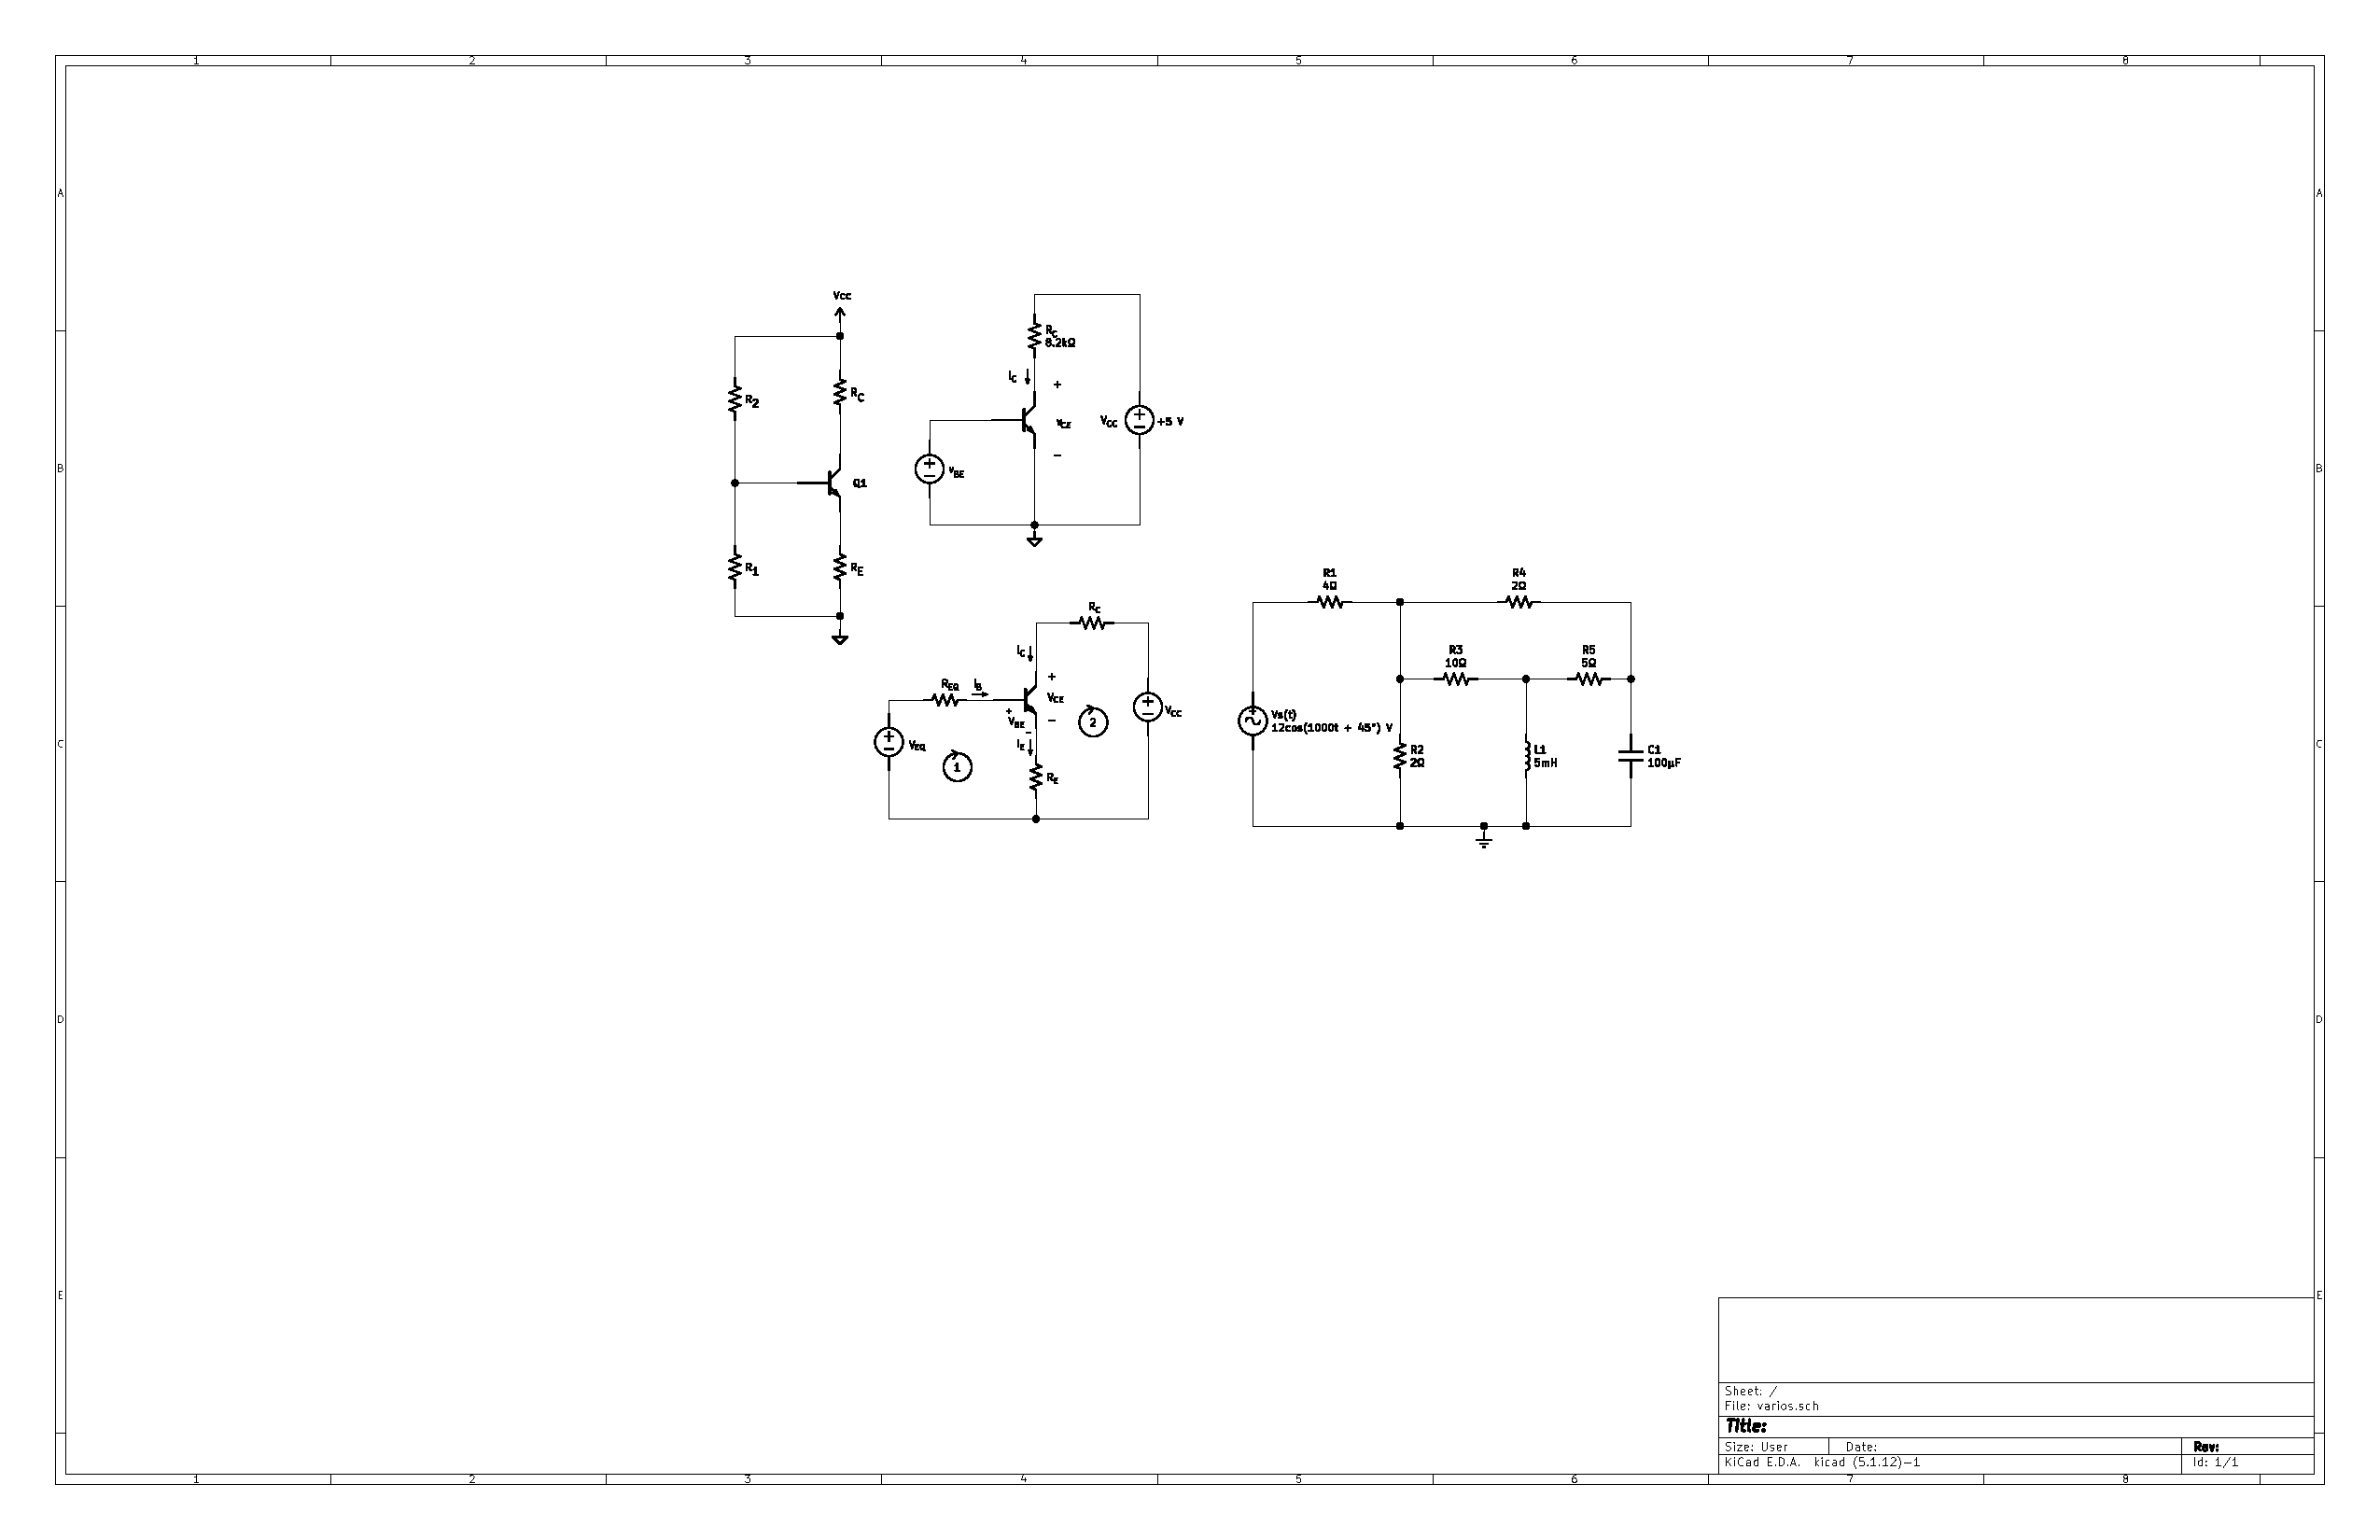
\includegraphics[scale=1.4,trim={16.4cm 18cm 21.4cm 5cm},clip]{varios}
	\caption{Red de polarización con 4 resistores.}
	\label{fig:figura1}
\end{figure}

\noindent La gráfica característica de transferencia de voltaje de este circuito aparece en la figura \ref{fig:figura2}. Para valores bajos de $v_{BE}$ el transistor se encuentra cerca de la región de corte y el voltaje de salida es $5\, V$, correspondiendo al número binario "1" en aplicaciones lógicas. Conforme $v_{BE}$ se incrementa alrededor de los $0.6 \,V$, la salida cae rápidamente y alcanza su  voltaje de "encendido" de $0.18\, V$ para $v_{BE}$ mayor a $0.8 \, V$. El BJT se encuentra ahora operando en su región de saturación y ese pequeño voltaje de encendido correspondería a un "0" en la lógica binaria.\\

Para regiones de amplificación, el punto Q se ubica en la región de alta pendiente (alta ganancia) de la característica de transferencia de voltaje (figura \ref{fig:figura2}). En este punto de operación, el transistor se encuentra operando en la región activa directa, región donde se pueden alcanzar una alta ganancia de voltaje, corriente y/o potencia.

%\pgfplotsset{width=9cm, compat=1.18}
\begin{figure}[H]
	\centering
	\begin{tikzpicture}
		\begin{axis}[
			title=Voltage Transfer Characteristic,
			xlabel={$v_{BE}$},
			ylabel={$v_{CE}$},
			ymin=0, ymax= 6,
			xmin=0, xmax=5,
			grid=major,
			scatter/classes={
				a = {mark=square*,draw=blue}
			},
			]
			\addplot [blue] table {plot1.dat};
			\addplot [scatter,only marks,scatter src=explicit symbolic,draw=blue,fill=white] coordinates {
				(0,5) [a]
				(0.63, 2.855) [a]
				(5.00, 0.064) [a]	
			};
			\node (A) at (0.5,5.5) {Q "off"};
			\node (B) at (1.5,2.85) {punto Q};
			\node (C) at (4.2,0.5) {Q "on"};
			\draw [->] (A) to (0.08,5.08);  
			\draw [->] (B) to (0.7,2.85); 
			\draw [->] (C) to (4.94,0.1); 
		\end{axis}   	 	
	\end{tikzpicture}
\caption{Grafica de la transferencia de voltaje.}
\label{fig:figura2}
\end{figure}

\begin{figure}[H]
	\centering
	\begin{tikzpicture}
		\begin{axis}[
			title=Voltage Transfer Characteristic,
			xlabel={$v_{BE}$},
			ylabel={$i_C$},
			ymin=0, ymax= 0.0009,
			xmin=0, xmax=7,
			grid=major,
			scatter/classes={
				a = {mark=square*,draw=blue}
			},
			]
			\addplot [blue] table [x=x, y=i1] {dato2.dat};
			\addplot [blue] table [x=x, y=i2] {dato2.dat};
			\addplot [blue] table [x=x, y=i3] {dato2.dat};
			\addplot [blue] table [x=x, y=i4] {dato2.dat};
			\addplot [blue] table [x=x, y=i5] {dato2.dat};
			\addplot [blue] table [x=x, y=i6] {dato2.dat};
			\addplot [blue] table [x=x, y=i7] {dato2.dat};
			\addplot [red, mark=*, mark options={fill=white}] coordinates{
				(0,609e-6)
				(5,0)
			};
			%\addplot [blue,domain=0:5,restrict y to domain=0:0.01] {5 - (8.2e3)*x};
		\end{axis}
	\end{tikzpicture}
	\caption{Grafica de la transferencia de voltaje.}
	\label{fig:figura5}
\end{figure}

\subsection*{Red de polarización de 4 resistores}
Debido a las relaciones exponenciales del BJT entre las corrientes y voltajes y su fuerte dependencia a la temperatura $T$, la forma de polarización utilizada en la figura \ref{fig:figura1} no representa una técnica práctica para establecer el punto de reposo. Uno de los mejores circuitos para estabilizar el punto Q de un transistor es la red de cuatro resistores que se muestra en la figura \ref{fig:figura3}

% trim={<left> <lower> <right> <upper>}
\begin{figure}[H]
	\centering
	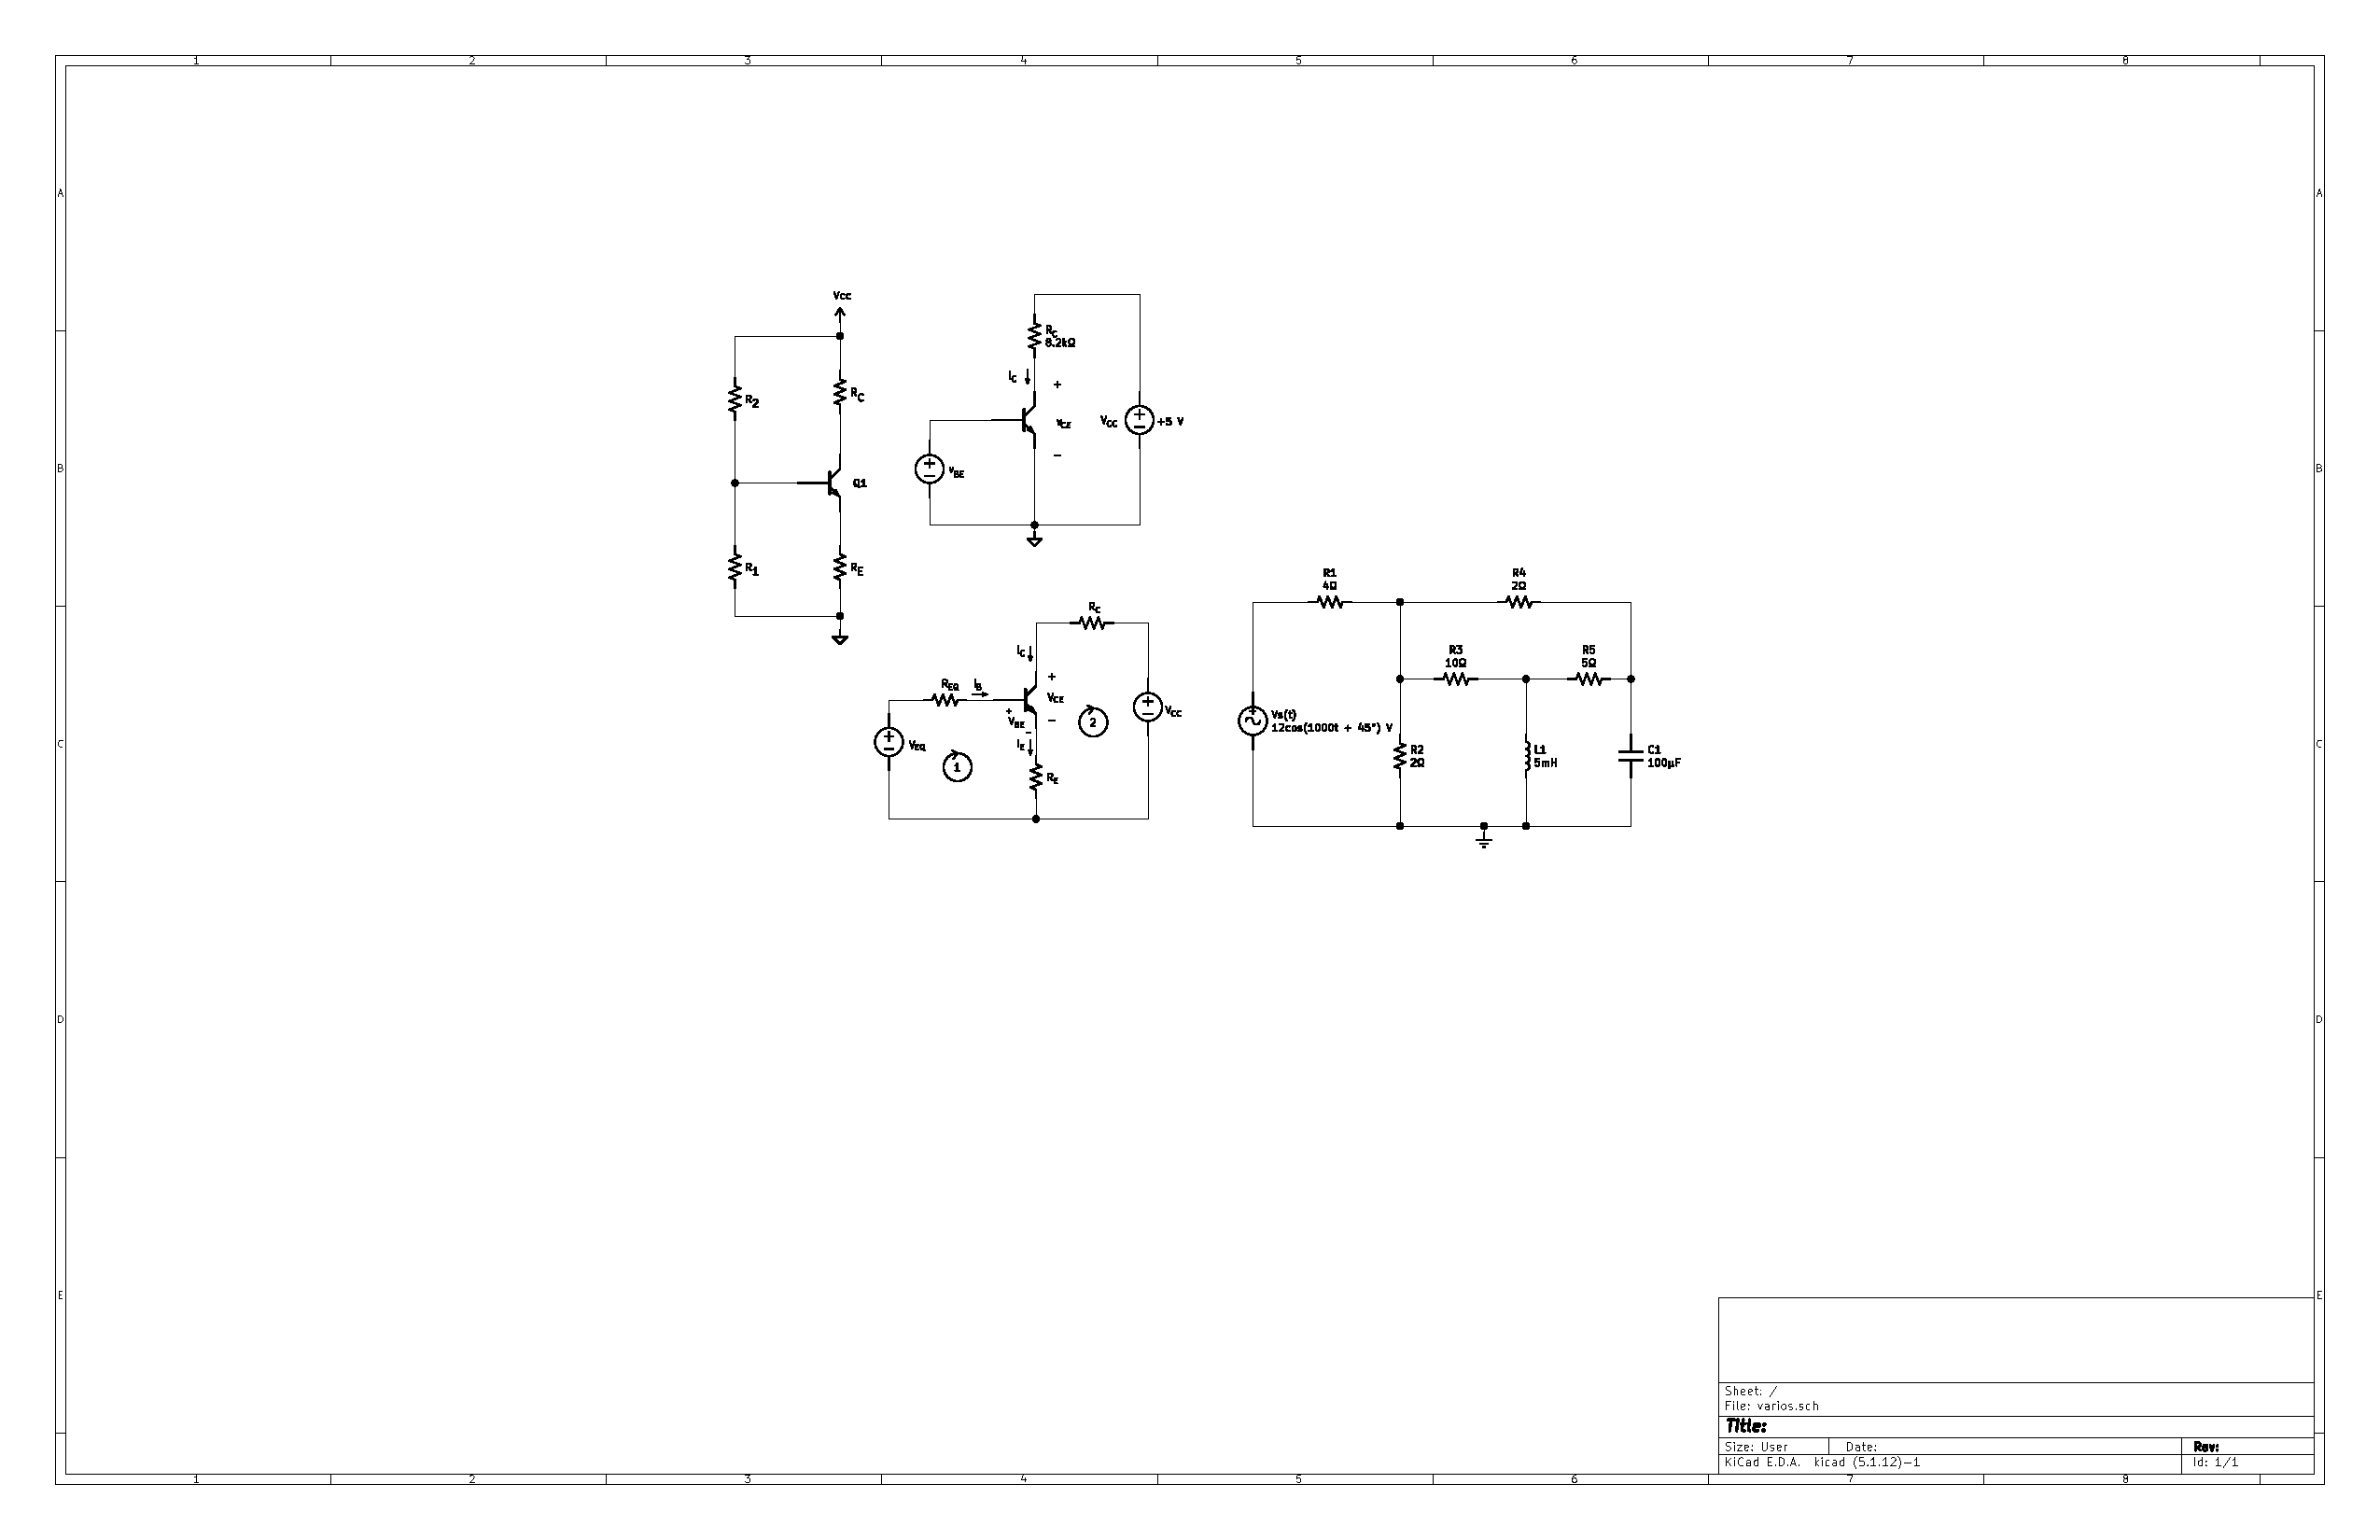
\includegraphics[scale=1.4,trim={13cm 16cm 27.3cm 5cm},clip]{varios}
	\caption{Red de polarización con 4 resistores.}
	\label{fig:figura3}
\end{figure}

\noindent $R_1$ y $R_2$ forman un divisor de voltaje resistivo a través de $V_{CC}$ y 0 V e intenta establecer un voltaje fijo en la base del transistor $Q_1$. $R_E$ y $R_C$ son usados para definir la corriente de emisor y el voltaje colector-emisor del transistor.

\noindent Nuestra meta es encontrar el punto Q del transistor: $(I_C, V_{CE})$. El primer paso en el análisis del circuito de la figura \ref{fig:figura3} es simplificar el circuito reemplazando la red de polarización de la base por su circuito equivalente de Thévenin como se muestra en la figura \ref{fig:figura4}. $V_{EQ}$ y $R_{EQ}$ están dados por

\begin{tcolorbox}[colback=red!5!white,colframe=red!75!black,arc=0mm,boxrule=0mm,width=(\linewidth+0.5cm),extrude right by=-1.5cm]
	\begin{equation}
		V_{EQ} = V_{CC} \frac{R_1}{R_1 + R_2} \,\,\,\,\,\,\,\,\,\, R_{EQ} = \frac{R_1 R_2}{R_1 + R_2}
	\end{equation}
\end{tcolorbox}

% trim={<left> <lower> <right> <upper>}
\begin{figure}[H]
	\centering
	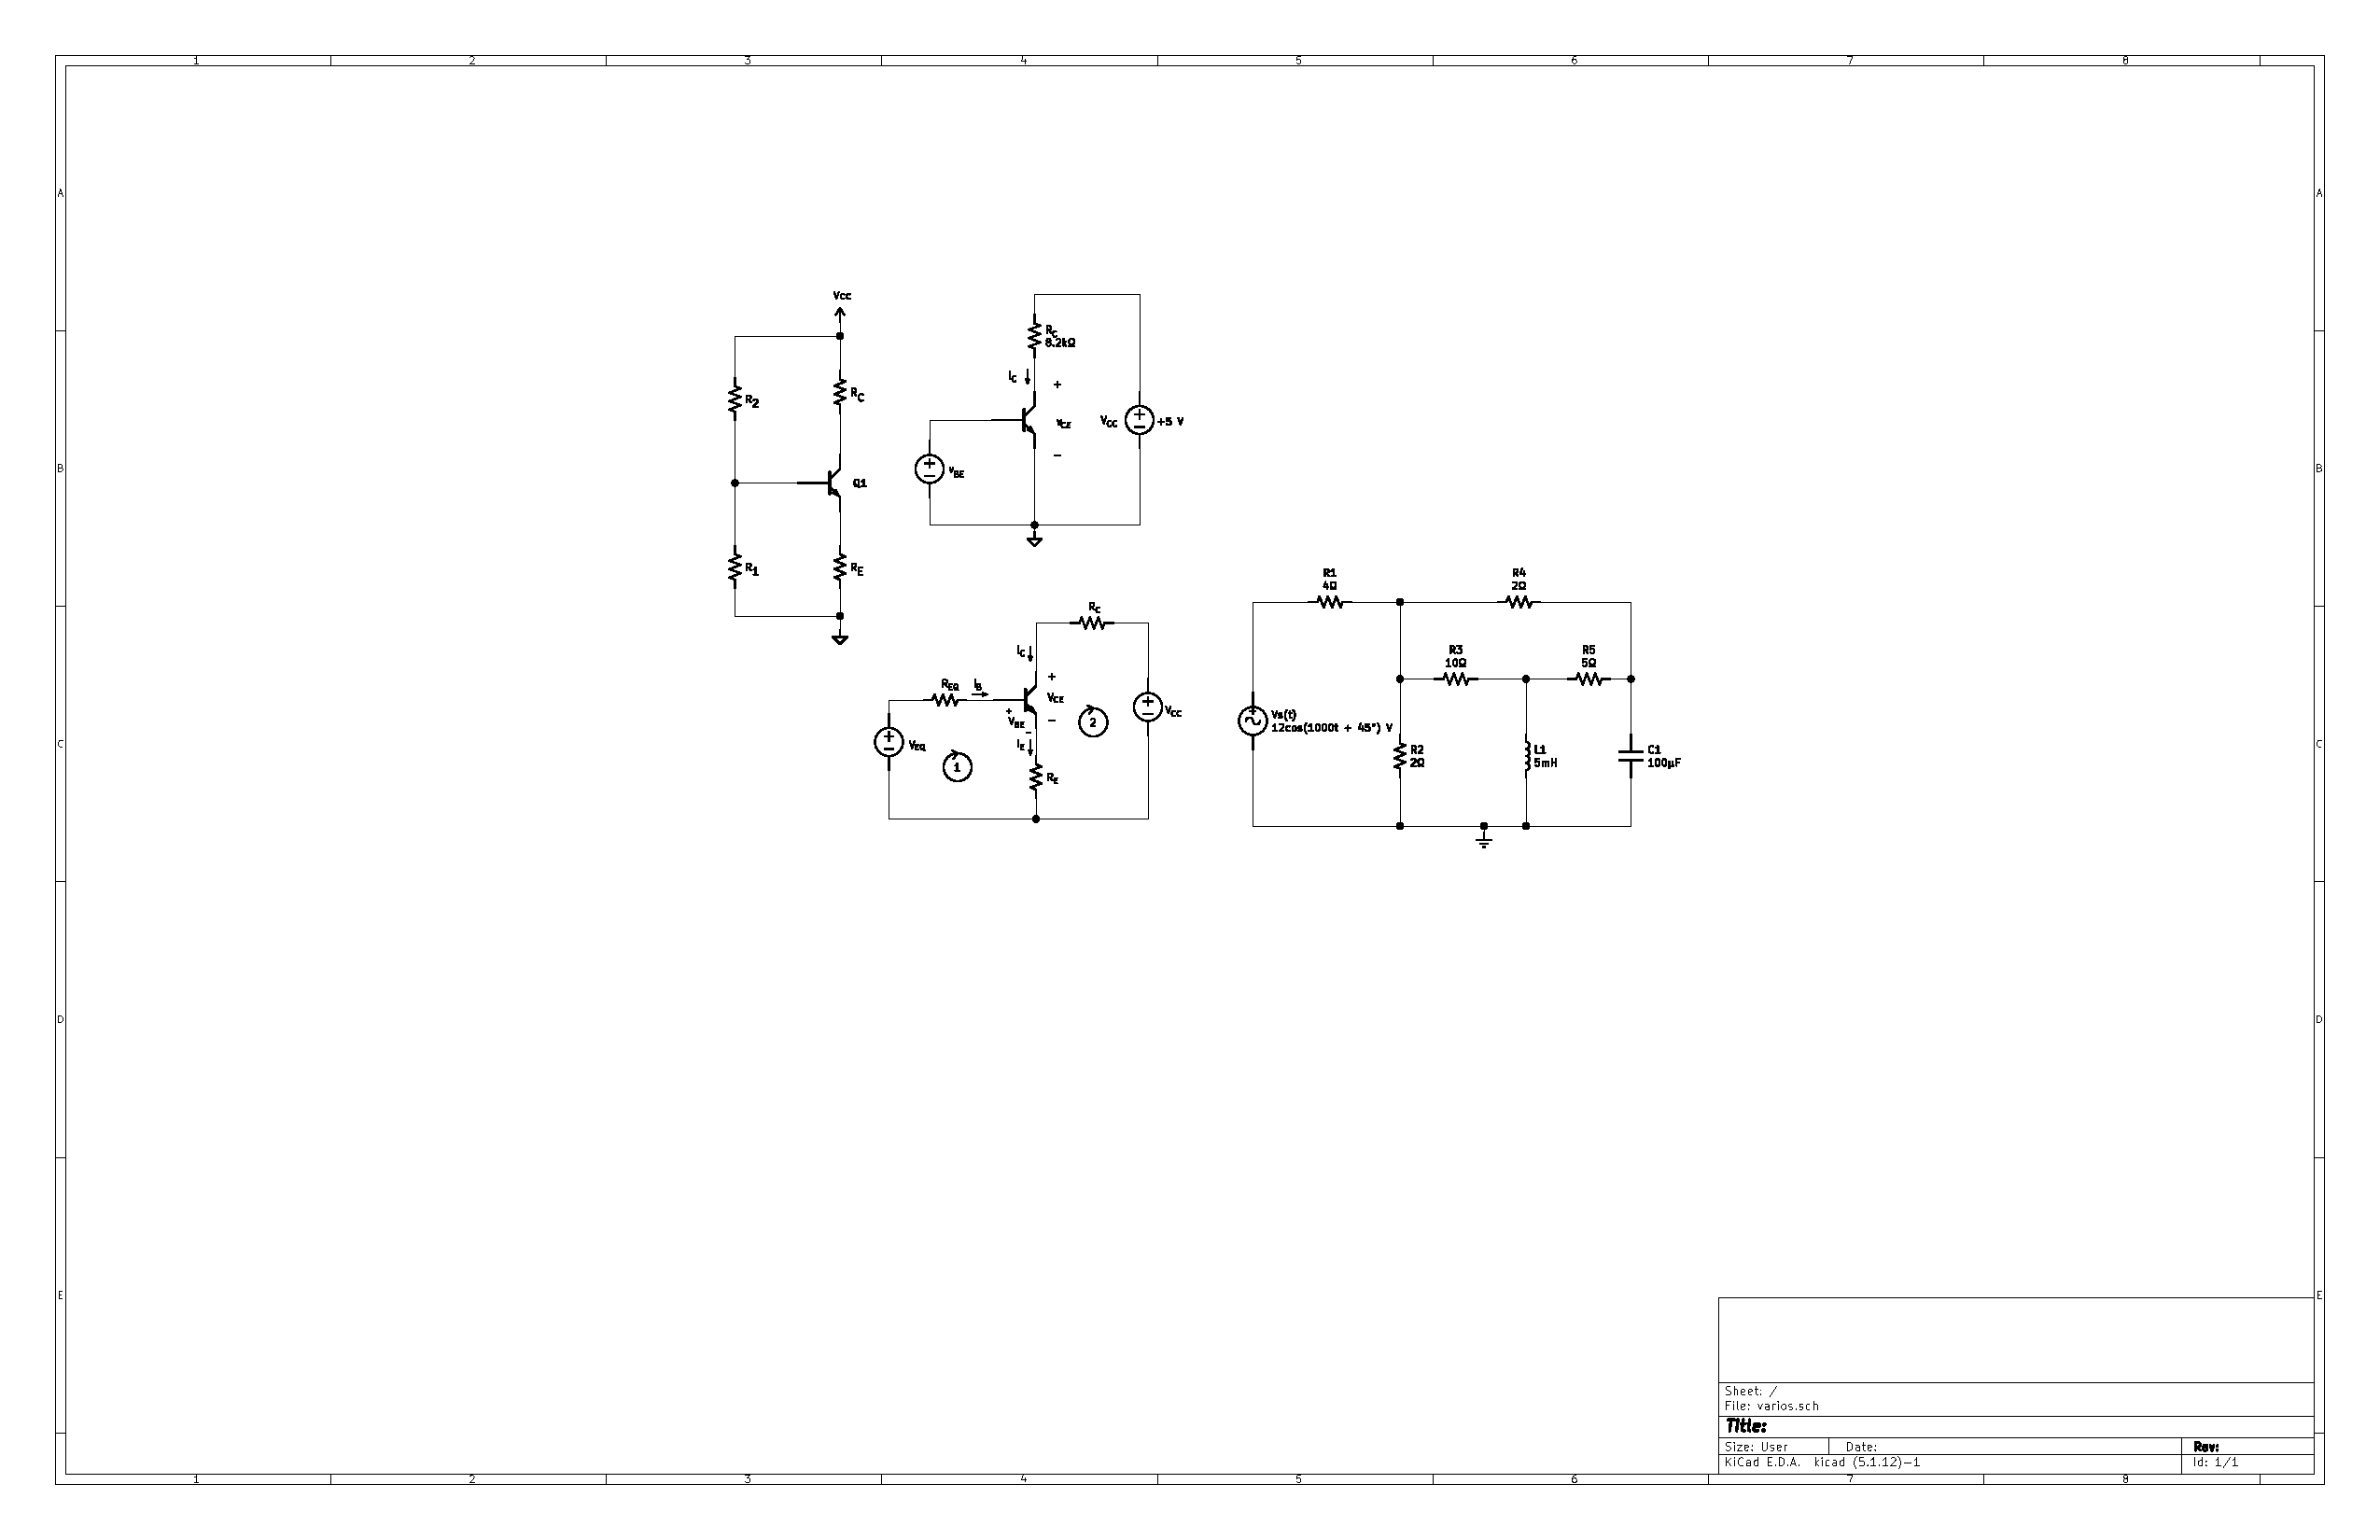
\includegraphics[scale=1.6,trim={15.5cm 13cm 21.4cm 10.9cm},clip]{varios}
	\caption{Equivalente de Thévenin para la red de polarización de 4 resistores.}
	\label{fig:figura4}
\end{figure}

\noindent Un análisis detalado de este circuito comienza con asumir una región de operación con el fin de simplificar las ecuaciones del modelo del BJT. Dado que la región de operación más común de este circuito es la región activa, asumiremos esta regiín para el análisis. Al usar la ley de tensión de Kirchhoff (LTK) alrededor del lazo 1 obtenemos:
\begin{align}
	V_{EQ} - R_{EQ}I_B - V_{BE} - R_EI_E = 0\nonumber\\
	V_{EQ} - R_{EQ}I_B - V_{BE} - (\beta + 1)I_BR_E = 0\nonumber
\end{align}

\noindent Al despejar $V_{EQ}$ obtenemos

\begin{align}
	V_{EQ} = R_{EQ}I_B + V_{BE} + (\beta + 1)I_BR_E
\end{align}

\noindent Al resolver para $I_B$ nos da
\begin{align}
	I_B = \frac{V_{EQ} - V_{BE}}{R_{EQ} + (\beta + 1)R_E} \,\,\,\,\,\, \text{donde} \,\,\,\,\,\, V_{BE} = V_T \ln \left( \frac{I_B}{I_S/\beta} + 1\right)
\end{align}

\noindent Desafortunadamente, al combinar estas expresionar obtenemos una ecuación trascendental. Sin embargo, si asumimos un valor apropiado de $V_{BE}$, entonces podremos encontrar las corrientes de colector y emisor usando nuestras relaciones auxiliares $I_C = \beta I_B$ y $I_E = (\beta + 1)I_B$:

\begin{tcolorbox}[colback=red!5!white,colframe=red!75!black,arc=0mm,boxrule=0mm,width=(\linewidth+0.5cm),extrude right by=-1.5cm]
	\begin{equation}
		I_C = \frac{\beta(V_{EQ} - V_{BE})}{R_{EQ} + (\beta + 1)R_E} = \frac{V_{EQ} - V_{BE}}{\frac{R_{EQ}}{\beta} + \frac{(\beta + 1)}{\beta}R_E}
	\end{equation}
\end{tcolorbox}

\noindent Y

\begin{tcolorbox}[colback=red!5!white,colframe=red!75!black,arc=0mm,boxrule=0mm,width=(\linewidth+0.5cm),extrude right by=-1.5cm]
	\begin{equation}
		I_E = \frac{(\beta + 1)(V_{EQ} - V_{BE})}{R_{EQ} + (\beta + 1)R_E} = \frac{V_{EQ} - V_{BE}}{ \frac{R_{EQ}}{\beta + 1} + R_E} 
	\end{equation}
\end{tcolorbox}

\noindent Para ganancias de corrientes muy altas $(\beta \gg 1)$, las ecuaciones (3), (4) y (5) pueden simplificarse de la siguiente manera:

\begin{align}
	I_E \cong I_C \cong \frac{V_{EQ} - V_{BE}}{ \frac{R_{EQ}}{\beta} + R_E} \,\,\,\,\,\, \text{con} \,\,\,\,\,\, I_B \cong \frac{V_{EQ} - V_{BE}}{R_{EQ} + \beta R_E}
\end{align}

\noindent Ahora que conocemos $I_C$, podemos usar el lazo 2 para encontrar el voltaje colector-emisor $V_{CE}$ 

\begin{align}
	R_E I_E + V_{CE} + R_C I_C - V_{CC} = 0\nonumber\\
	\frac{\beta + 1}{\beta}I_C R_E + V_{CE} + R_CI_C - V_CC = 0\nonumber\\
	\left( R_C + \frac{\beta + 1}{\beta} R_E \right)I_C + V_{CE} - V_{CC} = 0\nonumber
\end{align}

\noindent Al despejar para $V_{CE}$ obtenemos
\begin{tcolorbox}[colback=red!5!white,colframe=red!75!black,arc=0mm,boxrule=0mm,width=(\linewidth+0.5cm),extrude right by=-1.5cm]
	\begin{equation}
		V_{CE} = V_{CC} - I_C\left[ R_C + \left( \frac{\beta + 1}{\beta} \right)R_E \right]
	\end{equation}
\end{tcolorbox}

\noindent Nuevamente, ya que normalmente $(\beta \gg 1)$ la euación en (7) puede reemplazarse como 
\begin{align}
	V_{CE} \cong V_{CC} - I_C(R_C + R_E)
\end{align}

\noindent Para corroborar que la suposición de la región activa fue correcta, con el uso de la ecuación (7) calculamos el valor del voltaje de la unión base-colector, es decir:
\begin{align}
	V_{BC} = V_{BE} - V_{CE}
\end{align}

\noindent Así, si el resultado de la ecuación (8) es negativo, asumimos que el uso de la región activa fue correcta.


\end{document}
